\newpage
\section{Methods}

The following institutions' radiocarbon measurements (${\Delta^{14}C}$ and/or FM) 
were compared with the GNS Rafter Radiocarbon Laboratory (hereby shortened to "RRL") in turn, each elaborated upon in the following sections. Each intercomparison is tailored specifically to the type of data available between each institution. 

\subsection{RRL and Heidelberg University}
\subsubsection{Available Data}
\label{section:AvailableData}
\begin{figure}[h!]
  \centering
  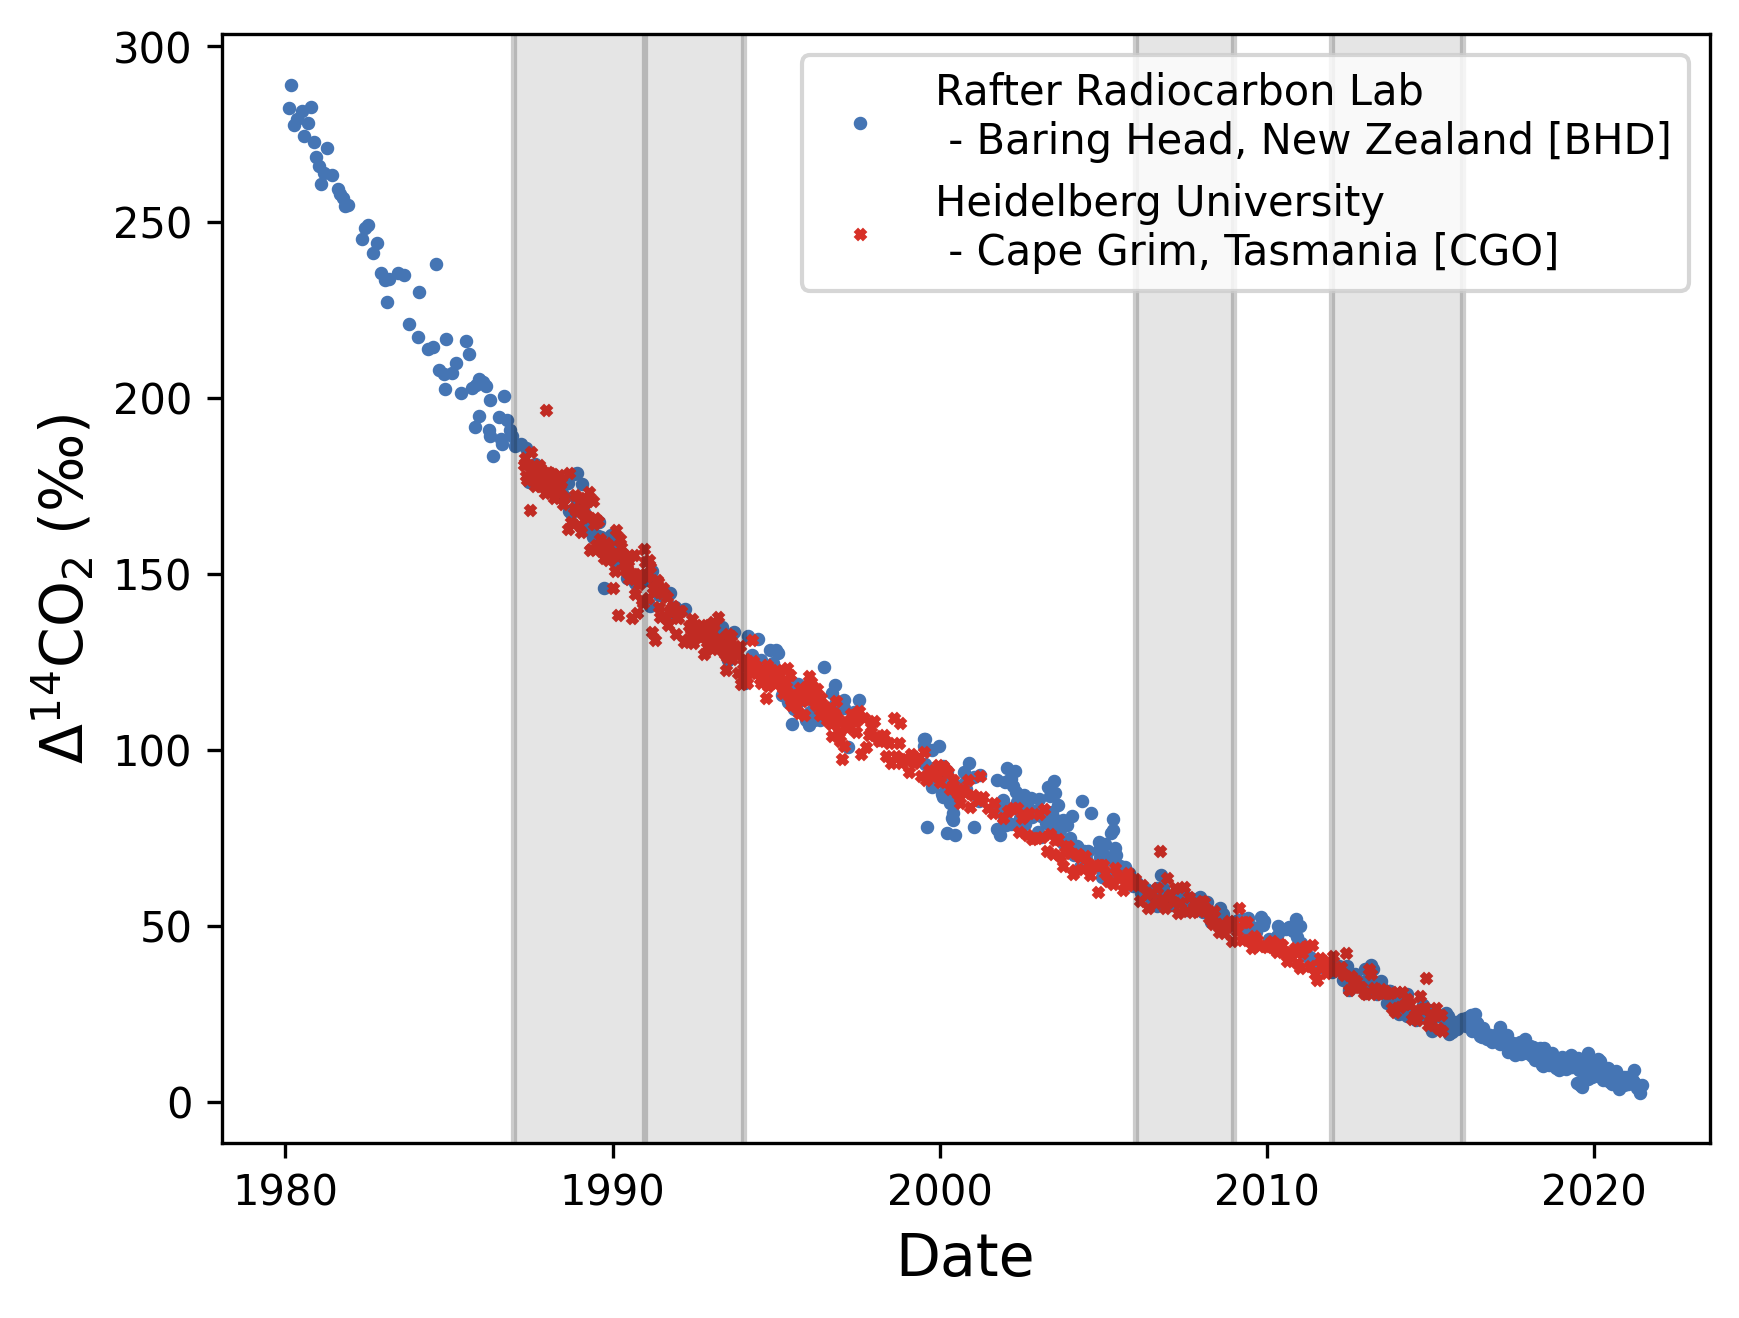
\includegraphics[width=12cm]{plots/new_test.png}
  \caption{Visual summary of available data used for intercomparison between Heidelberg University and Rafter Radiocarbon Lab. The four time intervals of focus are highlighted with background grey: 1987 - 1991, 1991 - 1994, 2006 - 2009, 2012 - 2016 }
  \label{fig:4timeintervals}
\end{figure}



% Give an overview of the data in the Wellington Record - but no detail about data treatment yet
\indent The RRL Wellington record is the earliest ${\Delta^{14}CO_{2}}$ dataset in the world, and the only one in the Southern Hemisphere to capture the "14C bomb-spike". Beginning in 1954 and still accumulating data, this record has seen changes in methods and sampling sites over the years, discussed in detail in ~\cite{turnbull2017}. Samples have been collected mainly via NaOH absorption; while Whole-air flask sampling was added as supplement since 1984. At RRL, sample ${CO_{2}}$ is extracted, graphitized~\cite{turnbull2015b} and ${\Delta^{14}CO_{2}}$ measured via accelerator mass spectrometry.\cite{turnbull2015b, ZONDERVAN201525}.

\indent The Heidelberg University Institute of Environmental Physics in affiliation with the ICOS Central Radiocarbon Laboratory operates a network of time-series stations measuring ${\Delta^{14}CO_{2}}$ sampled using the NaOH absorption method~\cite{levin1980, levin2010} and analyzed for ${^{14}CO_{2}}$ via decay counting~\cite{Kromer}. One of these stations, Cape Grim, Tasmania (CGO; 40.68S, 144.68E, 94 m a.s.l ~\cite{levin2010}), is a reasonable candidate through which to compare Heidelberg University to RRL ${\Delta^{14}CO_{2}}$ measurements through time. 

\indent CGO and Wellington observe a similar mixture of air from the Southern Ocean and Australia ~\cite{ziehn2014}, and have been found to be comparable in the past!\cite{turnbull2017}. Differences in seasonality and shifting air-mass origins with various contribution of fossil-CO2 are discussed in \cite{turnbull2017}, but will be ignored in this work which focuses on extracting longer-term trends (see section X).A short initial time-series indicates no measurable difference between the sites from 2017-2019 (See Figure \ref{fig:bhdvcgo}). \\

\indent The available data used to compare RRL and Heidelberg University can be seen at a glance in Figure\ref{fig:4timeintervals}). The Wellington record (1955-present) and CGO record (1987-2016) overlap for ~30 years.  
Certain intervals of data will be ignored.  
\indent It has been previously shown that data in the Wellington record sampled via NaOH absorption is anomalously different from CGO in the period between 1990 and 1993\cite{turnbull2017, levin2010}. In this time period, only Whole-air flask measurements are included for the Wellington Record.
\indent In 1995, RRL switched methods of ${\Delta^{14}C}$ measurement from gas-counting to AMS using an ENTandem system. In the period between 1995 and 2005, excess noise exists in the record, after which online $^{13}C$ measurement allowed for appropriate fractionation correction~\cite{turnbull2017, ZONDERVAN201525}, and significant decrease in noise. For this reason, the period between 1995 and 2005 is ignored. 
\indent RRL data in the period between 2009 and 2012 also is significantly offset from the otherwise consistency of the data; likely due to intermittent changes in NaOH absorption sampling techniques during this period. This period is therefore ignored for further intercomparison. 

\subsubsection{Intercomparison Method}
To extract long-term systematic offsets between institutions, and remove seasonality, the CCGCRV curve fitting procedure (~\cite{thoning1989}; www.esrl.noaa.gov/gmd/ccgg/mbl/crvfit/) is implemented similar to~\cite{turnbull2017}. We employ the "smooth" and "trend" functions of the CCGCRV algorithm. "Smoothed" data includes the results of the polynomial and harmonic fits of the data, and a long-term low-pass filter of 667 days. "Trended" data is similar; but retains the polynomial fit to the function and ignores harmonic components. 
Since the BHD and CGO data were not sampled on the same dates (i.e., they have an unequal number and value of x-components which impairs direct comparison of fitted data), the CCGCRV algorithm is programmed to output each smoothed/trended curve in 348 equal steps from 1987 to 2016 (12 samples/year), slightly underestimating the average sampling resolution of each dataset (CGO: 17 samples/year; BHD: 12.25 samples/year). By controlling the x-values of smoothed/trended data output from CCGCRV, the datasets can be compared. 
Error-estimates from the curve smoothing processes are obtained via a Monte-Carlo simulation, run to 10,000 iterations (for further details see Supplementary Information).


\subsection{RRL and Scripps Institute of Oceanography / Lawrence Livermore National Laboratory}

RRL and Scripps Institute of Oceanography / Lawrence Livermore National Laboratory (SIO/LLNL) are compared through measurement of the same standard materials, NWT3 and NWT4. NWT3 is a cylinder of air collected at Niwot Ridge, Colorado, USA in 2009. NWT4 is the same air, but spiked with 14C-free CO2. NWT3 and NWT4 are collected, maintained, and measured by INSTAAR for long-term repeatability assessments \cite{lehman2013allocation}. Through measurement collaboration, these standard were shared with LLNL and RRL. 
CO2 was produced from the sample air, combusted, extracted and measured similar to described in section \ref{section:AvailableData} ~\cite{turnbull2015b}.

At LLNL, NWT3 and NWT4 air was extracted according to techniques used for stable isotopic measurements at Scripps, independently tested for precision and accuracy \cite{guenther2001}, and measured on an HVEC FN Tandem accelerator at LLNL \cite{graven2007methods}.The measurements presented from LLNL were made between March and April of 2009, following the collaboration noted in \cite{lehman2013allocation}, while the measurements at RRL were made between 2013 and 2019. 



\subsection{RRL and Australian Nuclear Science and Technology Organisation (ANSTO)}

Intercomparability between RRL and ANSTO is assessed via measurement of the same Kauri tree-ring sampled from Eastbourne in Wellington, New Zealand. At RRL, the sample was pretreated to extract cellulose via solvent washes and subsequent oxidation according to~\cite{hua2000bomb, norris2015reconstruction}, and subsequently measured by AMS. 

%\subsection{University of Magallanes (NEED PERMISSION)}
  
%Intercomparability between University of Magallanes and RRL ${\Delta^{14}C}$ is assesed via measurements of tree-rings in Monte Tarn, Chile (53S. Samples from either institution were collected from the same site; but not the same tree. 
%\begin{itemize}
%	\item How was the sample prepared? Other details to add. 
%\end{itemize}

\subsection{Statistical Analyses}
For intercomparisons of non-stationary time-series, such as ANSTO and RRL tree-ring records and Heidelberg University and RRL atmospheric records, intercomparability is assessed using paired (relative) t-tests. Comparison with SIO/LLNL uses an independent t-test. In all cases, the null hypothesis is that no difference between the institutions exists. The hypothesis is rejected if p-values are <0.01 (these are displayed in Table X). Statistical calculations were made using the Python scipy.stats library (https://docs.scipy.org/doc/scipy/reference/stats.html).
